\chapter{Q-Metro}
Il \textbf{Q-Metro} misura le \textbf{impedenze} e i \textbf{fattori di merito/perdita} e si basa sul principio di \textbf{risonanza}:
  \begin{center}
    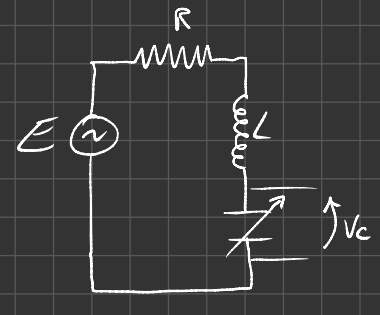
\includegraphics[width=0.40\textwidth]{Images/figure23.png}
  \end{center}
\begin{equation*}
    \w_0 L = \frac{1}{\w_0 C} \implies \w_0 = \sqrt{\frac{1}{LC}}
\end{equation*}
\begin{equation*}
    V_C = \underbrace{\frac{E}{R}}_{I} \cdot \frac{1}{\w_0 C} = E \frac{\w_0 L}{R} = E \cdot Q
\end{equation*}
Si dimostra che $\w_{max} = \w_0 \sqrt{1 - \frac{1}{2Q}}$ e se $Q > 10$ siamo in risonanza.\\ 
\section{Q-Metro con sostituzione tipo serie}
\begin{center}
    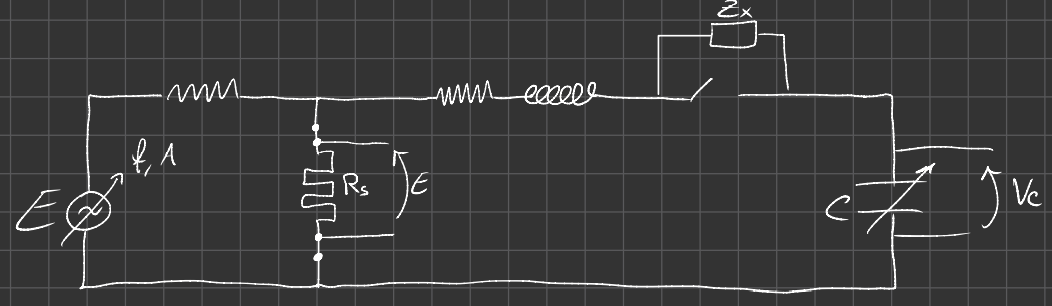
\includegraphics[width=\textwidth]{Images/figure24.png}
\end{center}
Dove $R_s$ è una resistenza molto piccola che serve per misurare E.\\ \\ \\ \\
\begin{center}
    \textbf{Prima misurazione (senza $Z_x$)}
\end{center}
\begin{equation*}
    X_L = X_{C_1} 
\end{equation*}
Che va in risonanza quando:
\begin{equation*}
    Q_1 = \frac{\w L}{R} = \frac{1}{\w R C_1} \implies R = \frac{1}{\w Q_1 C_1}
\end{equation*}
\begin{center}
    \textbf{Seconda misurazione (con $Z_x$)}
\end{center}
\begin{equation*}
    X_L + X_x = X_{C_2} \implies X_x = X_{C_2} - X_{C_1} = \frac{1}{\w C_2} - \frac{1}{\w C_1} = \frac{C_1 - C_2}{\w C_1 C_2} \implies
\end{equation*}
\begin{equation*}
    \implies Q_2 = \frac{1}{\w (R + R_x) C_2} \implies R+ R_x = \frac{1}{\w Q_2 C_2} \implies
\end{equation*}
\begin{equation*}
    \implies R_x = \frac{1}{\w Q_2 C_2} - \frac{1}{\w Q_1 C_1}
\end{equation*}
Da notare che, se $C_1 \approx C_2$ non va bene...\\
Va bene invece se $X_x$ ha $L >> 1$ oppure $C << 1$.